%卒論概要テンプレート ver. 4.0

\documentclass[uplatex,twocolumn,dvipdfmx]{jsarticle}
\usepackage[top=22mm,bottom=22mm,left=22mm,right=22mm]{geometry}
\setlength{\columnsep}{11mm}
\usepackage[T1]{fontenc}
\usepackage{txfonts}
\usepackage[expert,deluxe]{otf}
\usepackage[dvipdfmx,hiresbb]{graphicx}
\usepackage[dvipdfmx]{hyperref}
\usepackage{pxjahyper}
\usepackage{secdot}




%タイトルと学生番号,名前だけ編集すること
\title{\vspace{-5mm}\fontsize{14pt}{0pt}\selectfont ブロックチェーン技術を用いたマネジメント法の提案}
\author{\normalsize プロジェクトマネジメントコース 矢吹研究室 1442068 鈴木 博文}
\date{}
\pagestyle{empty}
\begin{document}
\fontsize{10.5pt}{\baselineskip}\selectfont
\maketitle





%以下が本文
\section{序論}\label{序論}

当研究では,急速に発展が拡大するブロックチェーン技術を,プロジェクトマネジメント(以下,PM)学科内の研究室において利用した際の利点・難点を調査する.

ファイナンスとテクノロジーを掛け合わせた造語である「フィンテック」の分野における企業買収や設立が昨年から緩和された\cite{touyou}.中でも世界的に流通が拡大しているのがビットコインを始めとした「仮想通貨」である.これが通貨として機能し,サービスが成り立つために必要な技術がブロックチェーンだ.

ブロックチェーンは「仮想通貨」だけでなく投資や投票など,他の分野でも活用が試みられている.

Jack du Rose氏が運営するColony社は,ブロックチェーンを会社経営・マネジメントに応用し,インターネット上での組織の自律的な運営を試みている\cite{wired}.

\section{目的}

ブロックチェーン技術を,マネジメントに応用した例を参考に,PM学科内の研究室において同技術を利用した際の利点・難点を研究する.出欠情報・プロジェクト内での作業時間・成績情報・経歴情報など,存在証明が必要とされるドキュメントを管理するプロトタイプを実装し記録改ざんの複雑化と存在証明の効率化を図る.

\section{手法}

ブロック作成に関する契約行動を自動実行出来る,スマート・コントラクトが構築可能なEthereumを利用し,以下の手順でプロトタイプ開発を行う.

\begin{enumerate}
\item コントラクトの管理者・認証組織・記録者本人のアカウントを作成する.
\item コントラクトにアクセスし,認証組織情報の入力,記録者の経歴を登録する.
\item 記録者本人により,閲覧許可の設定を行う.
\item 閲覧許可を得た組織が記録の閲覧を行う.
\end{enumerate}

\section{結果}

閲覧者と仮定した\verb|eth.accounts[3]|で登録した記録者の経歴を図\ref{code}の通り確認出来た.

\verb|contractObj.getPerson.call|によって記録者の氏名・生年月日・所属している組織を取得し,最終行で同スクリプトを実行して閲覧期限が切れた場合の実行結果も確認出来た.

%図の挿入
\begin{figure}[htb]
\centering
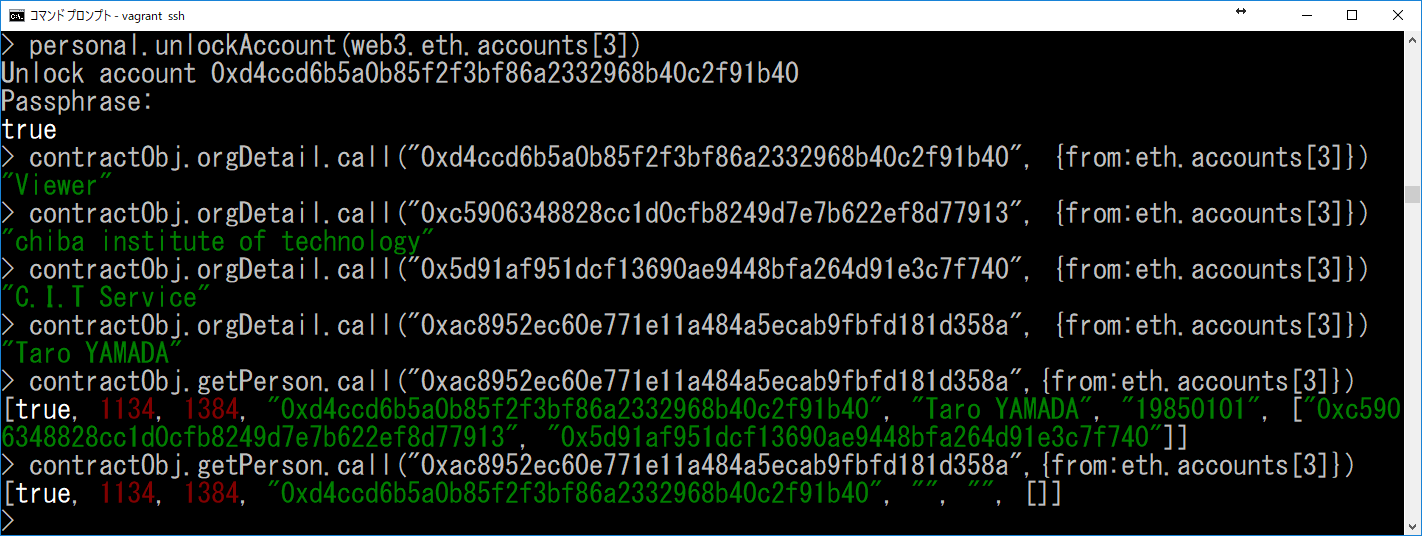
\includegraphics[width=7.7cm,clip]{code.png}
\caption{登録された経歴情報の取得結果}\label{code}
\end{figure}

\section{考察}

ブロックチェーンを用いた存在証明をスマート・コントラクトにて構築でき,PM学科内においても幅広く利用する価値があるのではないかと考えた.

電子記録の存在証明はプロジェクト内の成果物において利用することも重要であるため,構築したプロトタイプの強化も有用と考える.

\section{結論}

証明が必要となるドキュメントをブロックチェーンで管理することで,改ざんを複雑化しデータの信頼性を向上させることが出来た.

マネジメントに応用する点で独自性が低いため,具体的に利用する内容の検討が必要である.

\bibliographystyle{junsrt}
\bibliography{biblio}%「biblio.bib」というファイルが必要.

\end{document}
